\chapter{Software products}

\section{Project-based Software Engineering}
\textbf{Project-based software engineering} was the first form of software engineering. It starts from the desire of the customers, and at the end of the project you obtain software to be given to the user.

Developers usually try to transition from products originated from different customer to a single product that satisfy all types of customers. The problem with project-based software engineering was that the customer have to generate the requirements in a certain format about things that they generally don't understand. The customer doesn't think in terms of software requirements (requirements specify what is the software we need to implement), so it forces the customer to generate them. The requirements, also, are not static: they change each time we meet customers, because they understand what the software can do for them.

\begin{figure} [H]
    \centering
    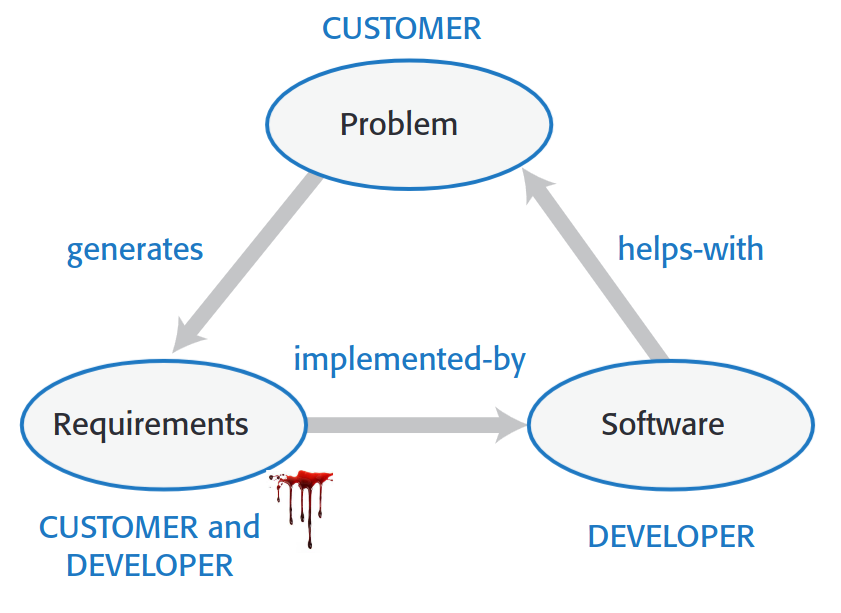
\includegraphics[width=0.6\textwidth]{images/Products/ProductsSE.png}
    \caption{Life cycle of project-based software engineering}
    \label{fig:ProductsSE}
\end{figure} 

\noindent 
For most business, users don't need customized software, but they need generalized software.

\section{Product-based Software Engineering}

In \textbf{product-based software engineering} the group of developers decides which are the software features, and how the software will change. The customer disappears from the cicle, so the developer choose which project they will build. The developers must identify features that meet the needs of the customers.

\begin{figure} [H]
    \centering
    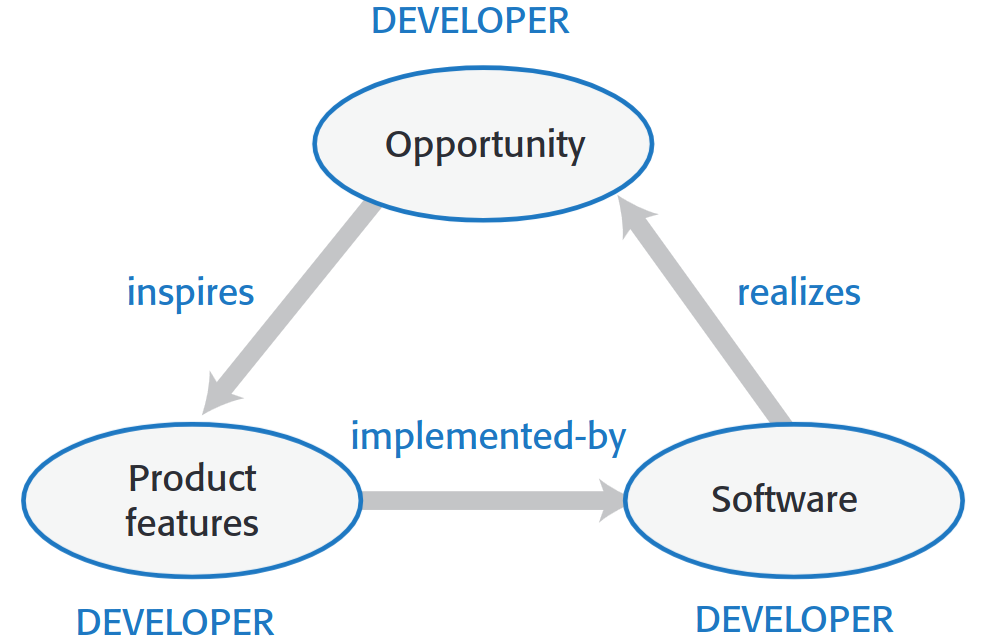
\includegraphics[width=0.6\textwidth]{images/Products/productbasedSE.png}
    \caption{Life cycle of product-based software engineering}
    \label{fig:productbasedSE}
\end{figure} 

One of the products based software engineering requirements is that we need to develop software quickly in order to not let someone else steal that market share. That's why time is critical, and that's why agile methods are used. \\

There are 3 types of \textbf{software execution models}: 
\begin{itemize}
    \item \textbf{Stand-alone execution}: The user interface, functionalities, and data are all stored on the user's computer. The vendor is responsible for creating and sending updates.
    \item \textbf{Hybrid execution}: Part of the application is on the end-user device (user interface, user data, and all updates from the vendor), and part is on the vendor's server (business logic and user data backups).
    \item \textbf{Software as a service} (SaaS): The user doesn't need to install anything (they just have an interface), meaning the program is hosted on the vendor's server. This makes it easier to manage and update the program without needing to distribute it. 
\end{itemize}

\begin{figure} [H]
    \centering
    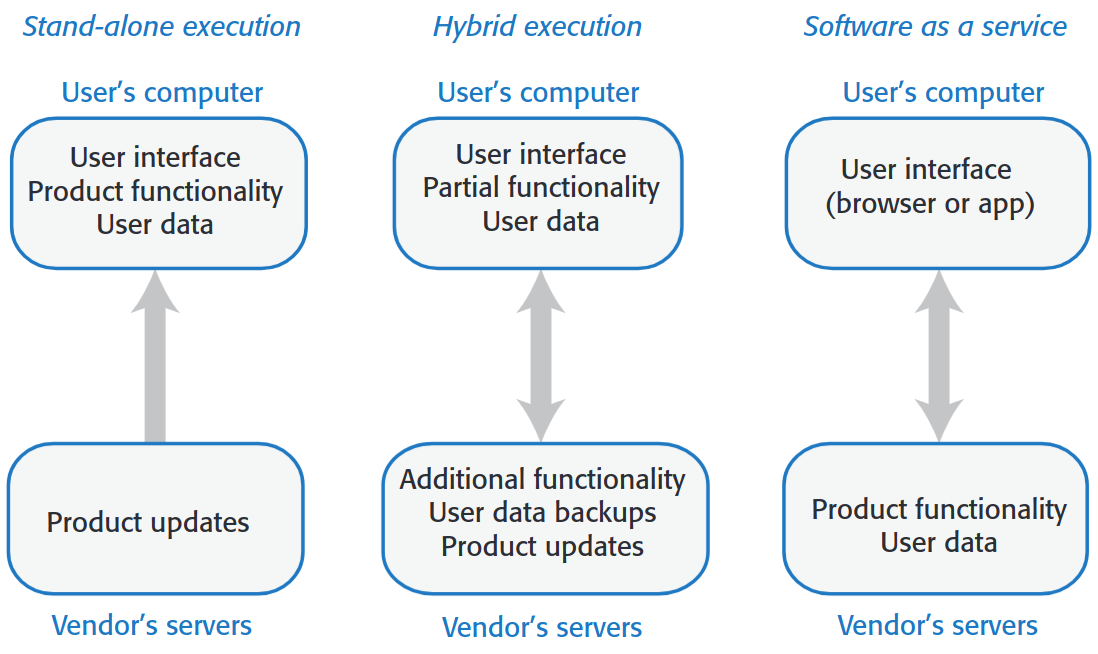
\includegraphics[width=0.66\textwidth]{images/Products/executionmodels.png}
    \label{fig:executionmodels}
    \caption{Execution models}
\end{figure} 

\section{Product vision}

For any new promising software program, there should be a \textbf{vision for the program}: \textcolor{green}{Who} are the targeted customers? \textcolor{brown}{What} is the product to be developed? \textcolor{red}{Why} should customers buy the product?

\noindent For programmers, it's easier to build cards with the following structure:
\newline \noindent \textcolor{green}{FOR (target customer)} \textcolor{green}{WHO (statement of the need or opportunity)}
\newline \noindent \textcolor{brown}{THE (product name) is a (product category)} \textcolor{brown}{THAT (key benefit, compelling reason to buy)}
\newline \noindent \textcolor{red}{UNLIKE (primary competitive alternative)} \textcolor{red}{OUR PRODUCT (statement of primary differentiation)}\\

These are the relevant aspects to building a product vision:
\begin{itemize}
    \item \textbf{Domain experience}: The product developers may work in a particular area (such as marketing and sales) and understand the software support they need. They may be frustrated by the deficiencies in the software they use and see opportunities for an improved system.
    \item \textbf{Product experience}: Users of existing software (such as word processing software) may identify simpler and better ways to provide comparable functionality and propose a new system to implement this. New products can also take advantage of recent technological developments (such as speech interfaces).
    \item \textbf{Customer experience}: Software developers may have extensive discussions with prospective customers to understand the problems they face, as well as constraints, such as interoperability, that limit their flexibility to buy new software. Developers also consider the critical attributes customers need in the software.
    \item \textbf{Prototyping and experimentation}: Developers may have an idea for software but need to develop a better understanding of the concept and what is involved in turning it into a product. Prototyping allows for the exploration of new ideas and feedback from customers (since customers think in terms of functionalities), guiding the path for the next prototype.
\end{itemize}

\section{Software product management}

The \textbf{Product Manager} must ensure that the development team implements features that deliver real value to customers. They must also find a balance between these three forces (we'll see how some Agile techniques help the Product Manager achieve these results):

\begin{itemize}
    \item \textbf{Business needs}: The entire product development process must be managed while considering business needs. The PM needs to ensure that the product satisfies the goals of both the customer and the company.
    \item \textbf{Customer experience}: Regularly gather feedback from customers to understand their experience with the product.
    \item \textbf{Technology constraints}: Consider the various technology constraints the company may have. The Product Manager must take into account the type of hardware and technology the customer already uses.
\end{itemize}

\begin{figure} [H]
    \centering
    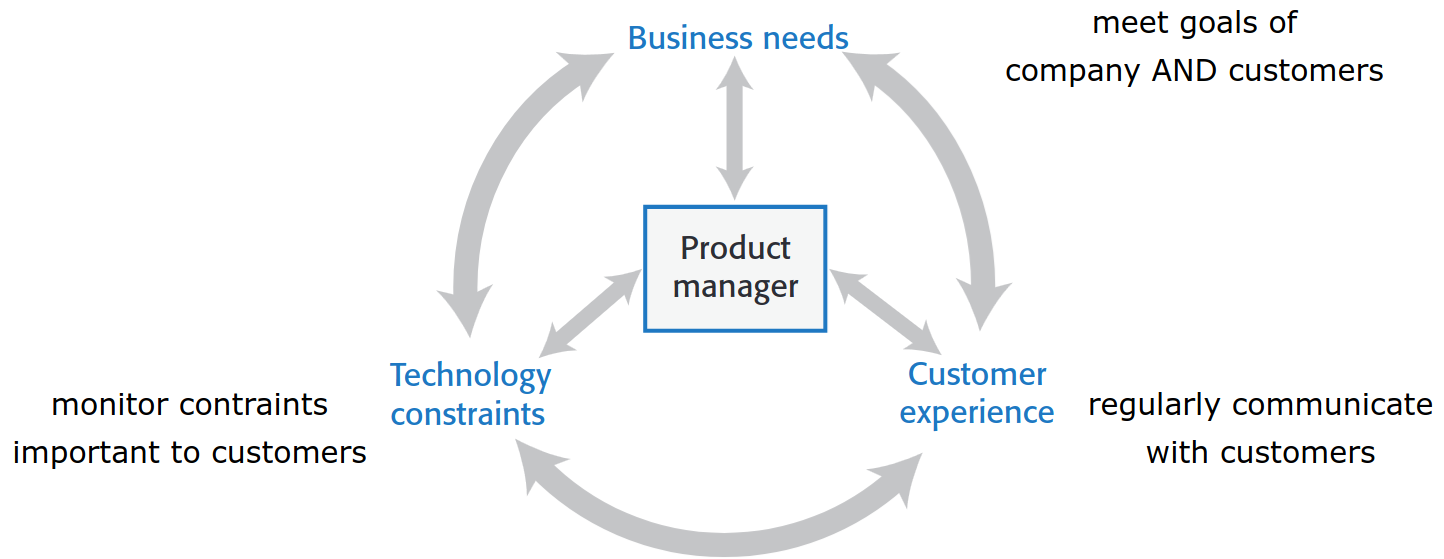
\includegraphics[width=0.73\textwidth]{images/Products/productmanager.png}
    \caption{Product Manager duties}
    \label{fig:productmanager}
\end{figure}

The Product Manager will have some \textbf{technical interactions} such as:
\begin{itemize}
    \item The \textbf{Product roadmap}, which includes setting goals, milestones, success criteria, and alternative paths in case the goals are not reached.
    \item \textbf{User stories and scenarios} to identify product features.
    \item The \textbf{Product backlog}, a to-do list for completing project development.
    \item \textbf{Acceptance testing}, which is used throughout the product lifecycle to verify that releases meet the set goals.
    \item \textbf{Customer testing}, which involves gathering feedback on usability and features.
    \item \textbf{UI design} to ensure simplicity and a natural user interface.
\end{itemize}

%he especially need to make sure that the product meets the goal of the customers. 1:00:00 for full image expl.